\documentclass[12pt,a4paper]{article}

\usepackage[utf8]{inputenc}
\usepackage[T1]{fontenc}
\usepackage[portuguese]{babel}
\usepackage{graphicx}
\usepackage{booktabs}
\usepackage{array}
\usepackage{float}
\usepackage{hyperref}
\usepackage{geometry}
\geometry{margin=2.5cm}

\graphicspath{{figures/}}

\title{Relatório de Acessibilidade Web\\
       \large Análise WAVE --- Perspectiva do Leitor de Tela}
\author{}
\date{\today}

\begin{document}

\maketitle
\tableofcontents
\newpage

%% ─────────────────────────────────────────────────────────────
\section{Visão Geral}

\begin{table}[htbp]
  \centering
  \caption{Resumo de acessibilidade — todas as páginas}
  \label{tab:summary_all}
  \small
  \begin{tabular}{llcrrrrrr r}
\toprule
Fluxo & Página & AIM & Elem. & Erros & Contraste & Alertas & \% prob. & LS Crít. & LS Alto \\
\midrule
T3: Receita Federal & Receita Federal & 7.000000 & 608 & 17 & 8 & 40 & 10.700000 & 2 & 0 \\
T3: Receita Federal & Atendimento Presencial & 8.400000 & 478 & 5 & 0 & 20 & 5.200000 & 2 & 0 \\
T3: Receita Federal & Unidades Minas Gerais & 9.000000 & 479 & 5 & 0 & 20 & 5.200000 & 2 & 0 \\
T3: Receita Federal & Unidades Belo Horizonte & 9.100000 & 473 & 5 & 0 & 13 & 3.800000 & 2 & 0 \\
T3: Receita Federal & Unidades De Atendimento & 5.600000 & 64 & 6 & 11 & 28 & 70.300000 & 2 & 1 \\
T4: IBGE Censo & Ibge & 6.200000 & 240 & 7 & 18 & 33 & 24.200000 & 4 & 4 \\
T4: IBGE Censo & Resultados Censo2022 & 3.900000 & 336 & 38 & 60 & 85 & 54.500000 & 14 & 0 \\
T5: Mapa de Empresas & Mapa De Empresas & 8.600000 & 518 & 8 & 0 & 12 & 3.900000 & 2 & 0 \\
T2: Painel de Monitoramento & Governo Digital & 7.700000 & 626 & 11 & 0 & 33 & 7.000000 & 2 & 2 \\
T2: Painel de Monitoramento & Estrategias EGovernanca & 8.500000 & 457 & 5 & 1 & 16 & 4.800000 & 2 & 0 \\
T2: Painel de Monitoramento & Transformacao Digital & 7.800000 & 480 & 5 & 10 & 20 & 7.300000 & 2 & 0 \\
T2: Painel de Monitoramento & Central De Qualidade & 7.900000 & 480 & 5 & 10 & 16 & 6.500000 & 2 & 0 \\
T2: Painel de Monitoramento & Painel De Monitoramento & 7.900000 & 465 & 5 & 9 & 16 & 6.500000 & 2 & 0 \\
T1: Consulta CPF & Inicio Consultar Cadastro CPF & 8.500000 & 425 & 6 & 0 & 18 & 5.600000 & 2 & 2 \\
T1: Consulta CPF & Formulario Consulta CPF & 5.400000 & 62 & 5 & 11 & 22 & 61.300000 & 2 & 0 \\
T1: Consulta CPF & comprovante Situacao CPF & 6.000000 & 55 & 4 & 9 & 23 & 65.500000 & 1 & 0 \\
\bottomrule
\end{tabular}
\end{table}


\begin{figure}[htbp]
  \centering
  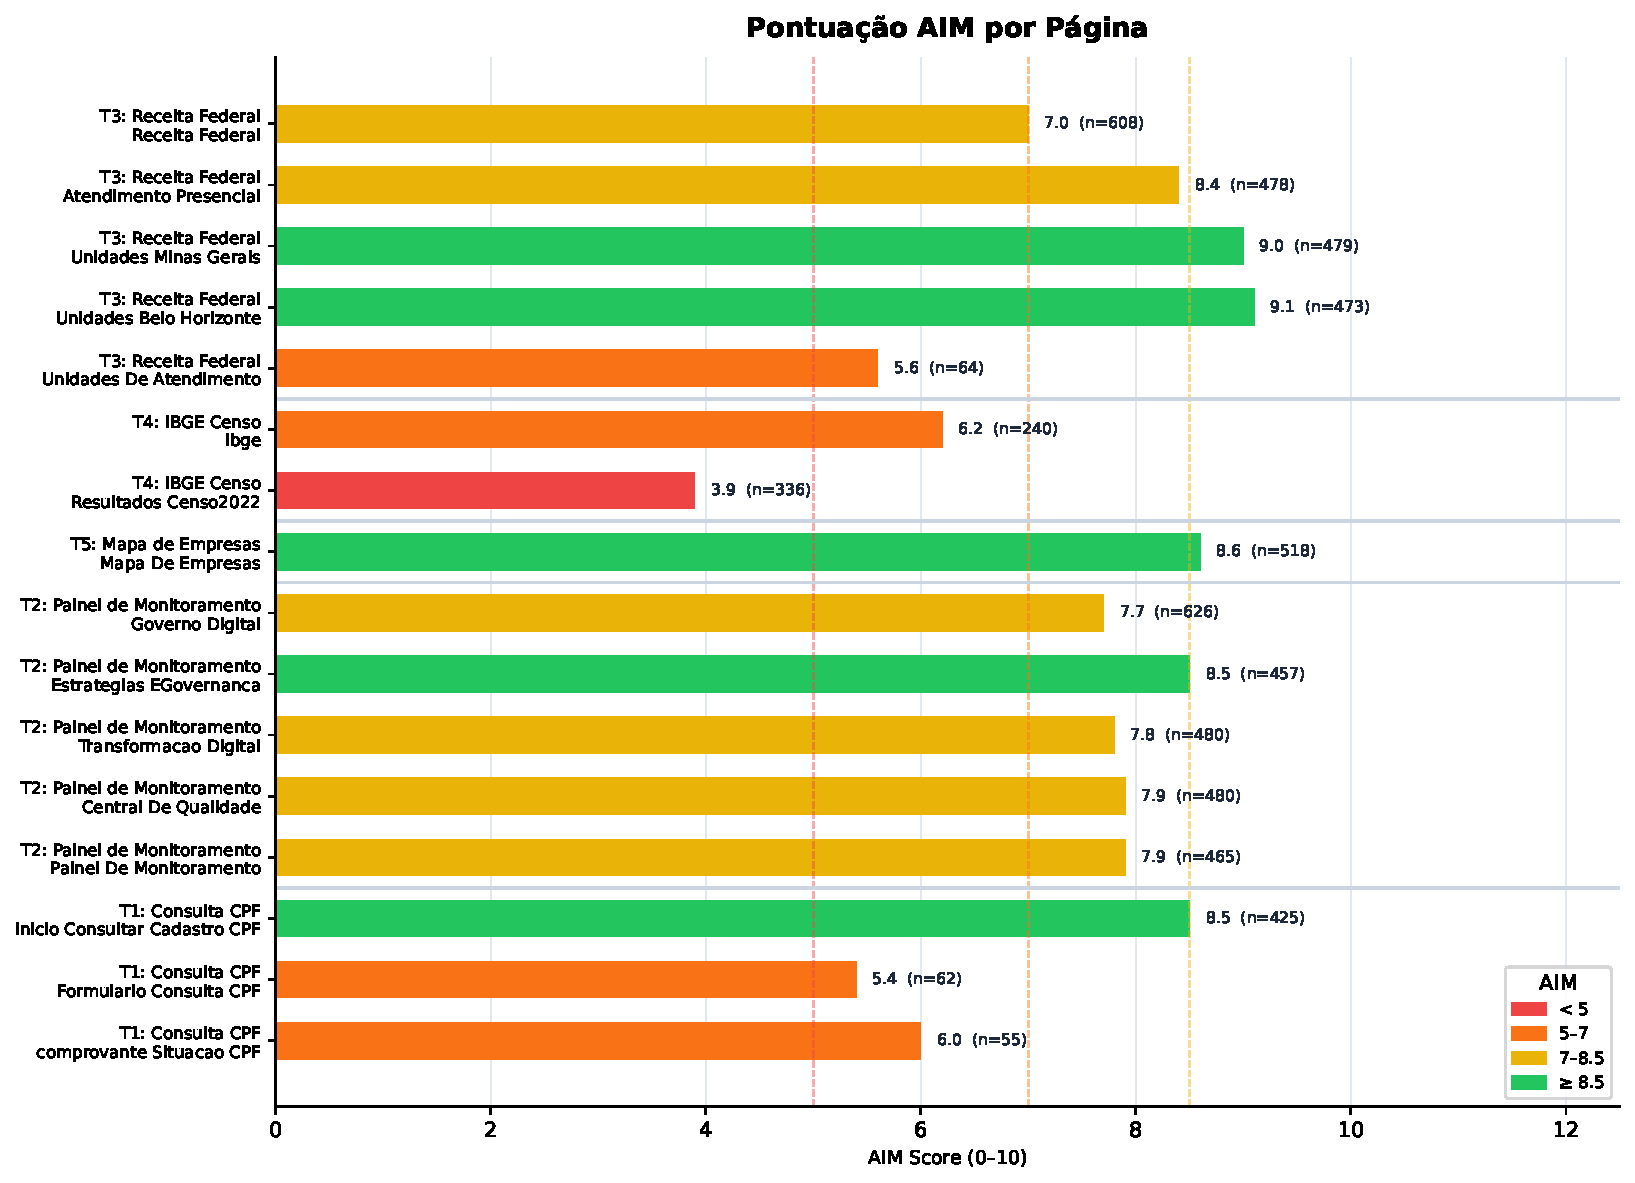
\includegraphics[width=\linewidth]{figures/aim_all_pages}
  \caption{Pontuação AIM por página (escala 0--10, maior é melhor).
           O valor \textbf{n} indica o total de componentes detectados pelo WAVE,
           usado como proxy do tamanho da página.
           Linhas tracejadas delimitam as faixas de qualidade em 5, 7 e 8{,}5.}
  \label{fig:aim_all}
\end{figure}

\begin{figure}[htbp]
  \centering
  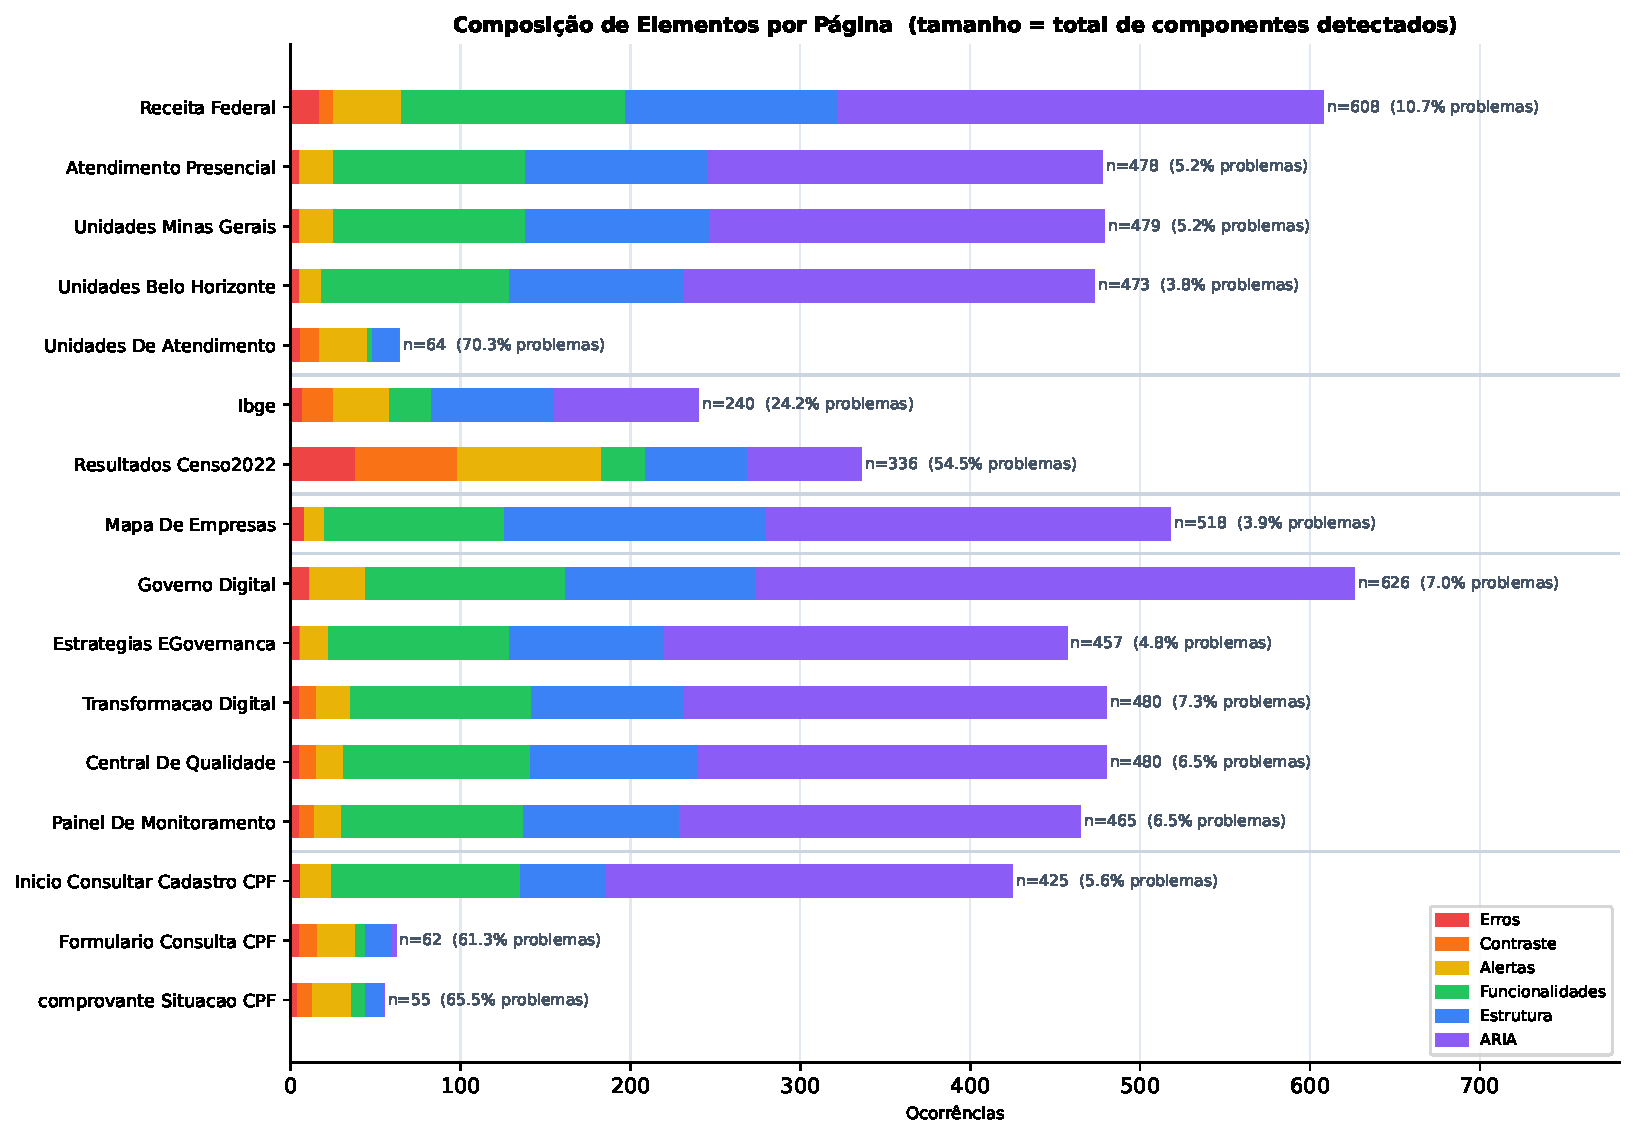
\includegraphics[width=\linewidth]{figures/elements_all_pages}
  \caption{Composição de todos os elementos detectados por página.
           A proporção de elementos negativos (erros, contraste, alertas)
           sobre o total é indicada como \emph{\% prob.} e permite comparar
           páginas de tamanhos diferentes.}
  \label{fig:elements_all}
\end{figure}

\begin{figure}[htbp]
  \centering
  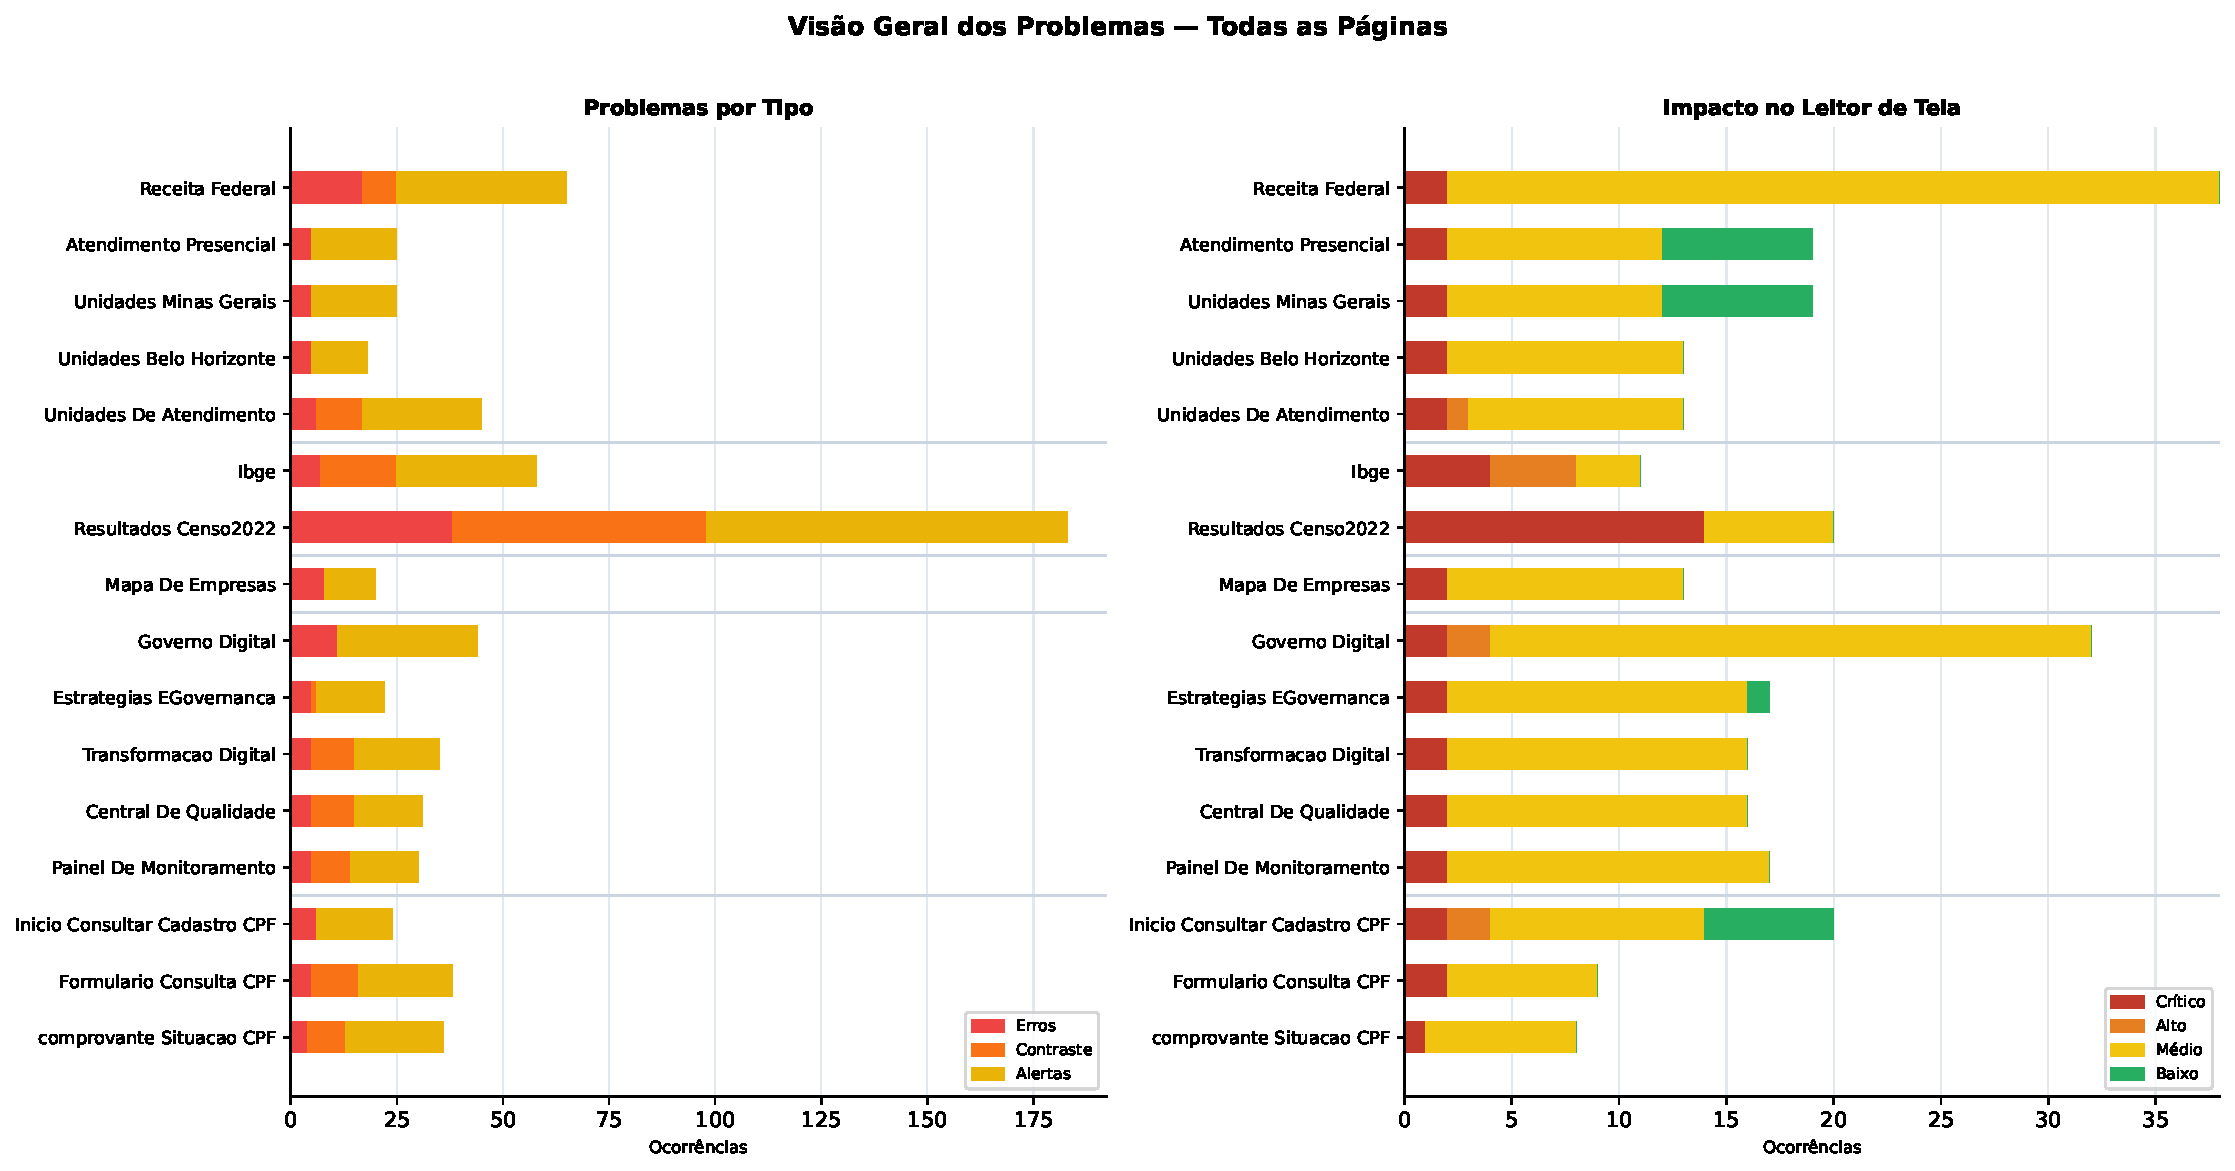
\includegraphics[width=\linewidth]{figures/issues_overview}
  \caption{Visão geral dos problemas: tipos de erro (esquerda) e
           impacto para usuários de leitores de tela (direita).}
  \label{fig:issues_overview}
\end{figure}

\begin{figure}[htbp]
  \centering
  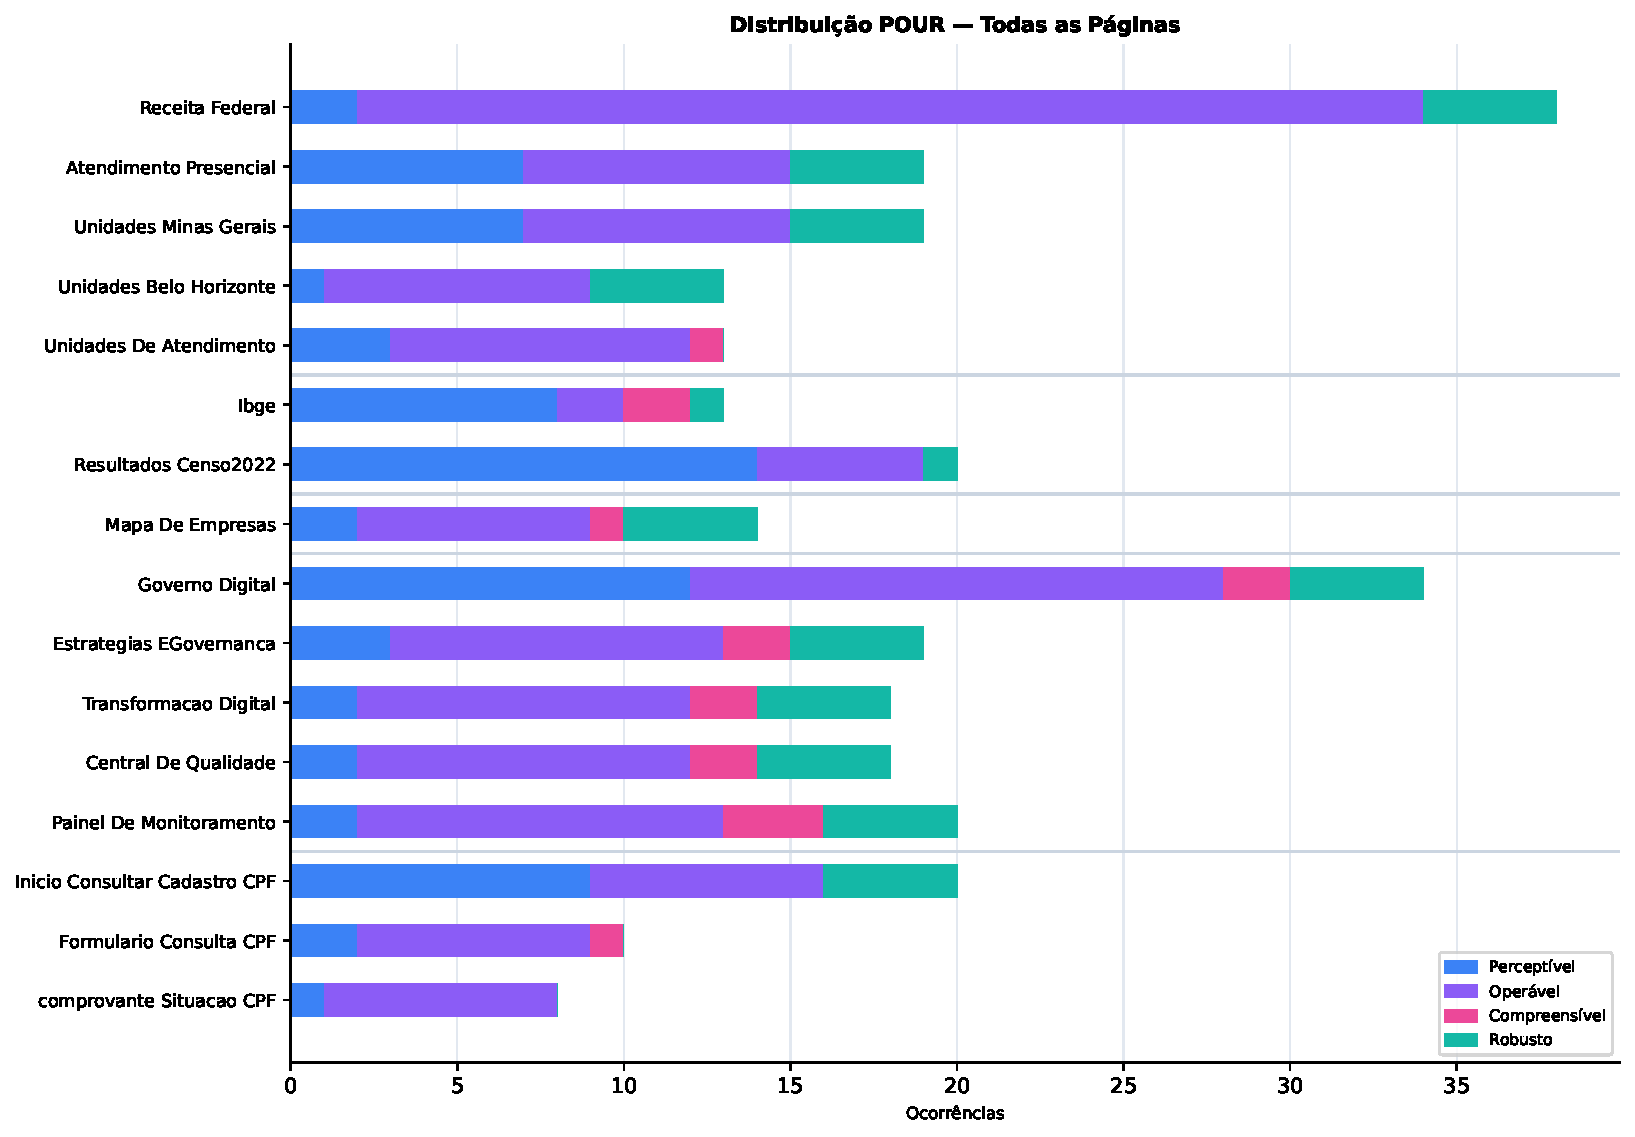
\includegraphics[width=\linewidth]{figures/pour_all_pages}
  \caption{Distribuição dos problemas pelas quatro dimensões WCAG (POUR).}
  \label{fig:pour_all}
\end{figure}

%% ─────────────────────────────────────────────────────────────
\section{Análise por Fluxo}


\subsection{T3: Receita Federal}

\begin{table}[htbp]
  \centering
  \caption{Métricas por página — T3: Receita Federal}
  \label{tab:flow_t3_receita_federal}
  \small
  \begin{tabular}{lcrrrrrrrrrr}
\toprule
Página & AIM & Elem. & \% prob. & Erros & Contraste & Alertas & Func. & Estrutura & ARIA & LS Crít. & LS Méd. \\
\midrule
Receita Federal & 7.000000 & 608 & 10.700000 & 17 & 8 & 40 & 132 & 125 & 286 & 2 & 36 \\
Atendimento Presencial & 8.400000 & 478 & 5.200000 & 5 & 0 & 20 & 113 & 108 & 232 & 2 & 10 \\
Unidades Minas Gerais & 9.000000 & 479 & 5.200000 & 5 & 0 & 20 & 113 & 109 & 232 & 2 & 10 \\
Unidades Belo Horizonte & 9.100000 & 473 & 3.800000 & 5 & 0 & 13 & 111 & 103 & 241 & 2 & 11 \\
Unidades De Atendimento & 5.600000 & 64 & 70.300000 & 6 & 11 & 28 & 3 & 16 & 0 & 2 & 10 \\
\bottomrule
\end{tabular}
\end{table}


\begin{figure}[htbp]
  \centering
  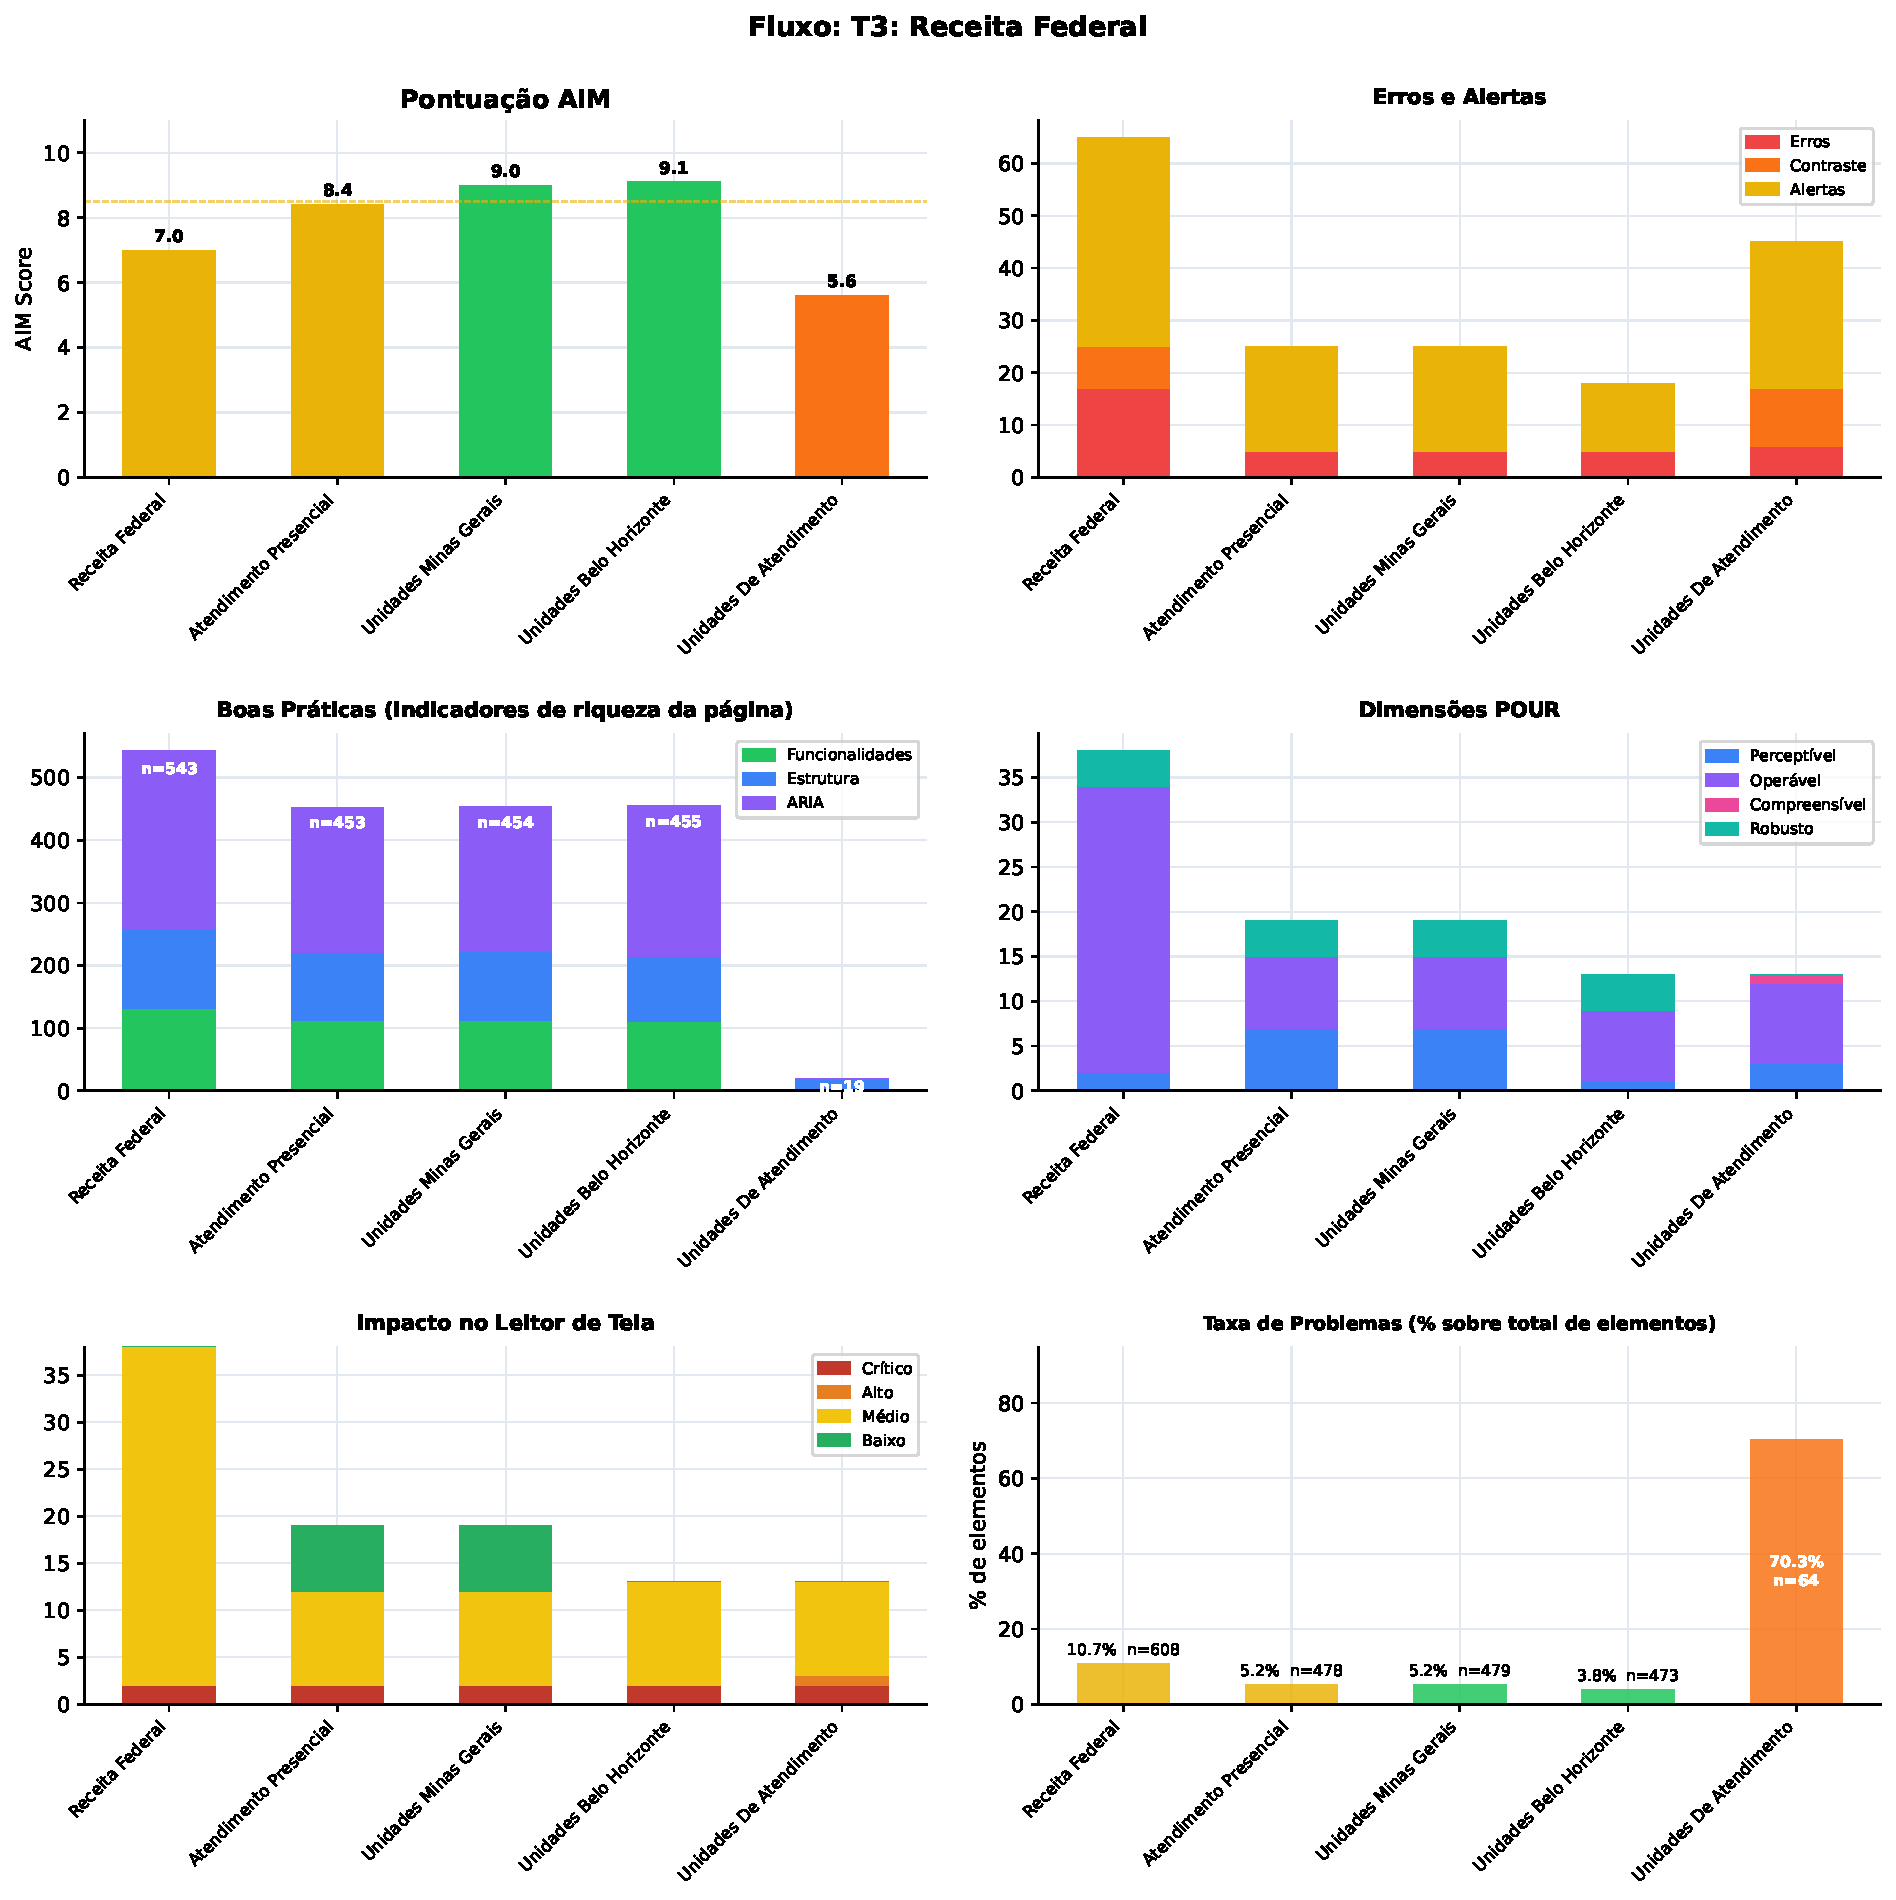
\includegraphics[width=\linewidth]{figures/flow_t3_receita_federal}
  \caption{Métricas de acessibilidade — T3: Receita Federal}
  \label{fig:flow_t3_receita_federal}
\end{figure}


\subsection{T4: IBGE Censo}

\begin{table}[htbp]
  \centering
  \caption{Métricas por página — T4: IBGE Censo}
  \label{tab:flow_t4_ibge_censo}
  \small
  \begin{tabular}{lcrrrrrrrrrr}
\toprule
Página & AIM & Elem. & \% prob. & Erros & Contraste & Alertas & Func. & Estrutura & ARIA & LS Crít. & LS Méd. \\
\midrule
Ibge & 6.200000 & 240 & 24.200000 & 7 & 18 & 33 & 25 & 72 & 85 & 4 & 3 \\
Resultados Censo2022 & 3.900000 & 336 & 54.500000 & 38 & 60 & 85 & 26 & 60 & 67 & 14 & 6 \\
\bottomrule
\end{tabular}
\end{table}


\begin{figure}[htbp]
  \centering
  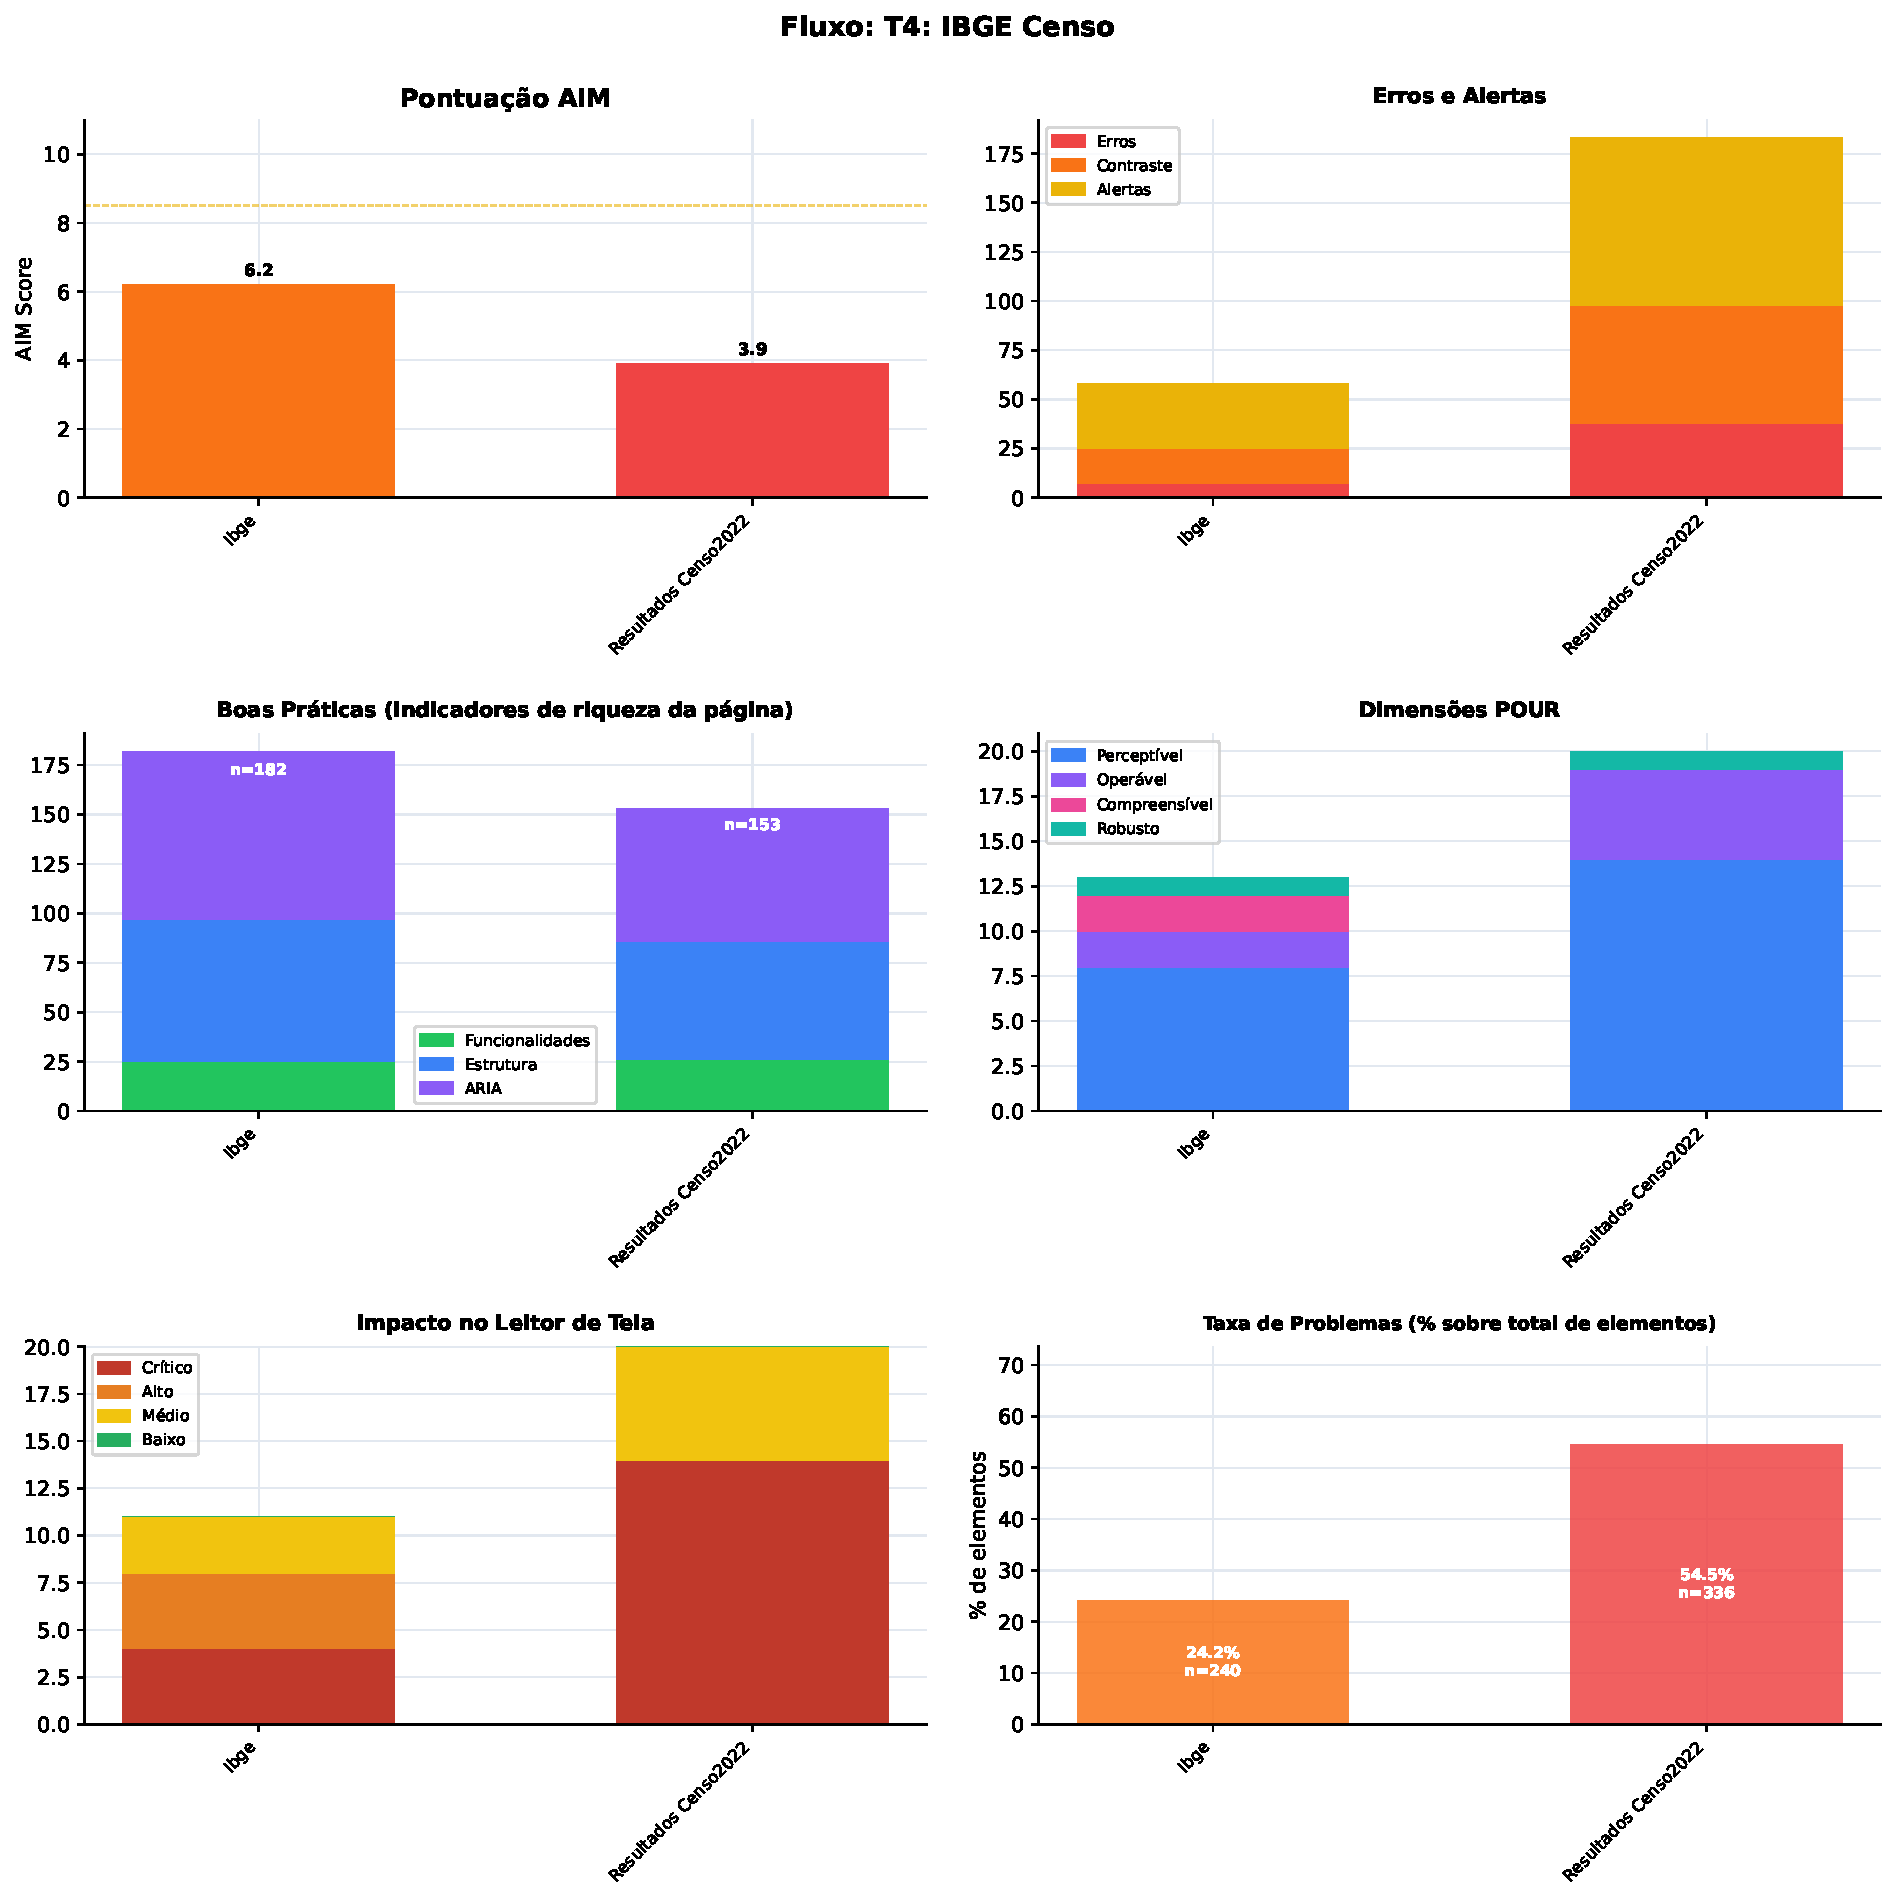
\includegraphics[width=\linewidth]{figures/flow_t4_ibge_censo}
  \caption{Métricas de acessibilidade — T4: IBGE Censo}
  \label{fig:flow_t4_ibge_censo}
\end{figure}


\subsection{T5: Mapa de Empresas}

\begin{table}[htbp]
  \centering
  \caption{Métricas por página — T5: Mapa de Empresas}
  \label{tab:flow_t5_mapa_de_empresas}
  \small
  \begin{tabular}{lcrrrrrrrrrr}
\toprule
Página & AIM & Elem. & \% prob. & Erros & Contraste & Alertas & Func. & Estrutura & ARIA & LS Crít. & LS Méd. \\
\midrule
Mapa De Empresas & 8.600000 & 518 & 3.900000 & 8 & 0 & 12 & 106 & 154 & 238 & 2 & 11 \\
\bottomrule
\end{tabular}
\end{table}


\begin{figure}[htbp]
  \centering
  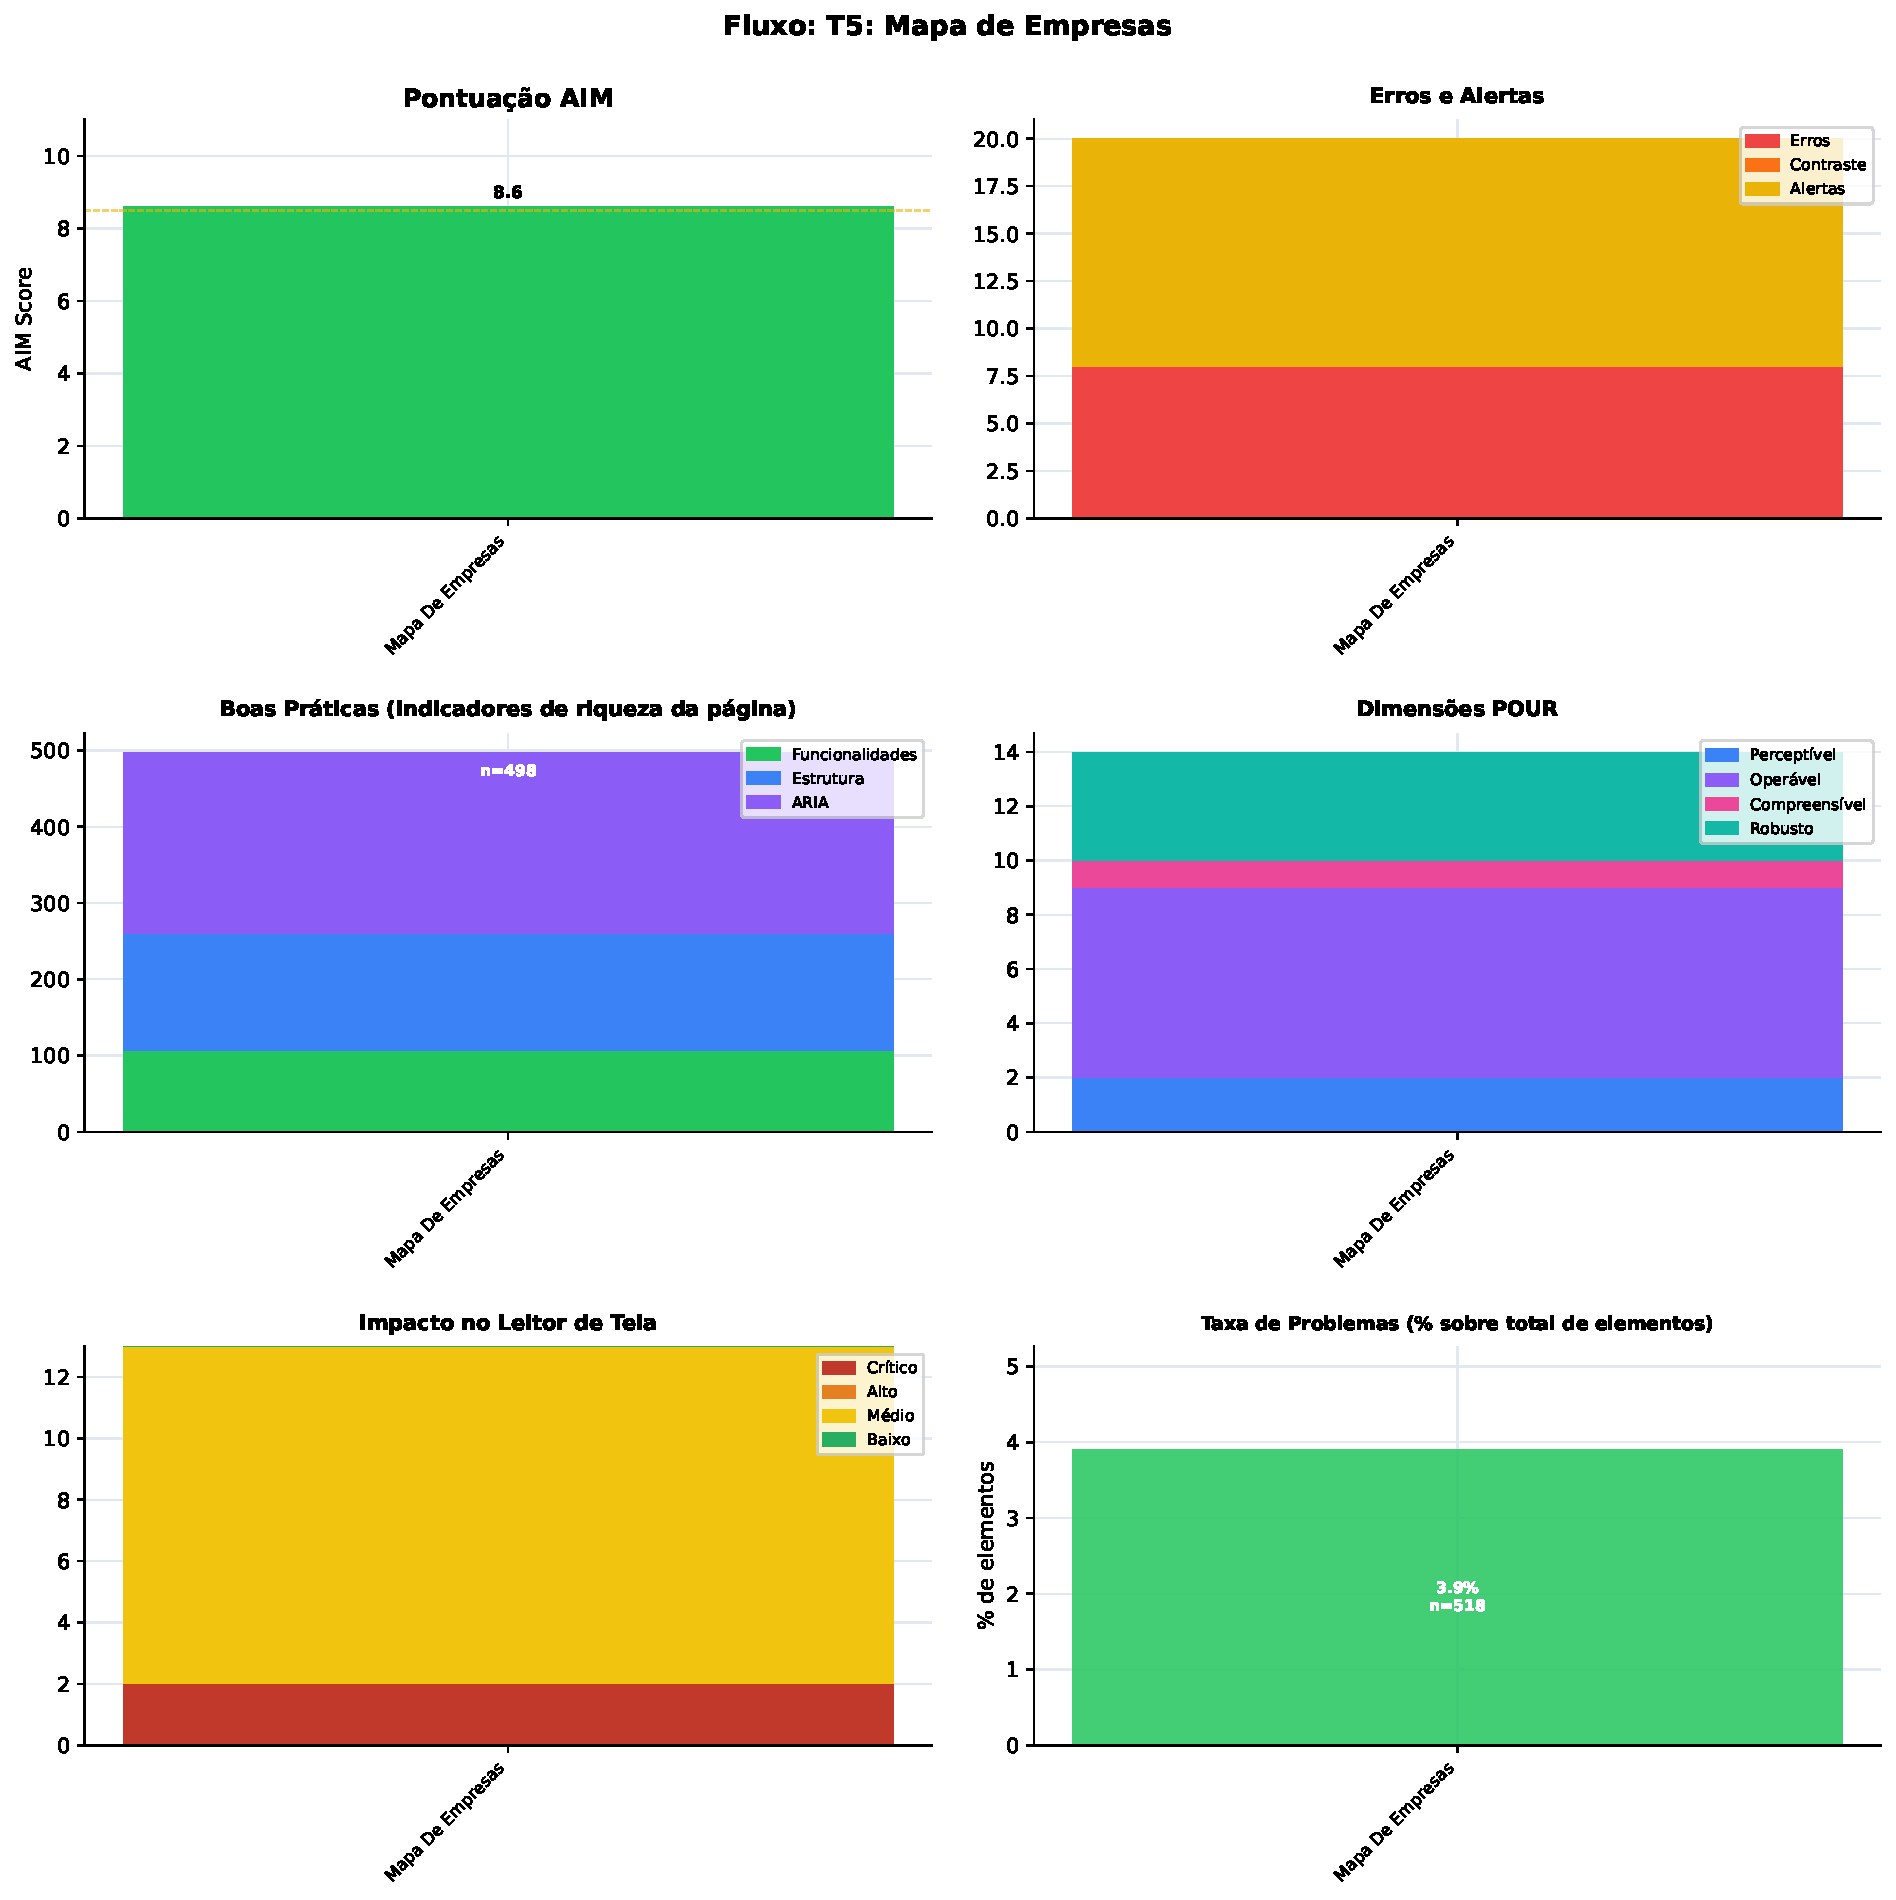
\includegraphics[width=\linewidth]{figures/flow_t5_mapa_de_empresas}
  \caption{Métricas de acessibilidade — T5: Mapa de Empresas}
  \label{fig:flow_t5_mapa_de_empresas}
\end{figure}


\subsection{T2: Painel de Monitoramento}

\begin{table}[htbp]
  \centering
  \caption{Métricas por página — T2: Painel de Monitoramento}
  \label{tab:flow_t2_painel_de_monitoramento}
  \small
  \begin{tabular}{lcrrrrrrrrrr}
\toprule
Página & AIM & Elem. & \% prob. & Erros & Contraste & Alertas & Func. & Estrutura & ARIA & LS Crít. & LS Méd. \\
\midrule
Governo Digital & 7.700000 & 626 & 7.000000 & 11 & 0 & 33 & 118 & 112 & 352 & 2 & 28 \\
Estrategias EGovernanca & 8.500000 & 457 & 4.800000 & 5 & 1 & 16 & 107 & 91 & 237 & 2 & 14 \\
Transformacao Digital & 7.800000 & 480 & 7.300000 & 5 & 10 & 20 & 107 & 90 & 248 & 2 & 14 \\
Central De Qualidade & 7.900000 & 480 & 6.500000 & 5 & 10 & 16 & 110 & 99 & 240 & 2 & 14 \\
Painel De Monitoramento & 7.900000 & 465 & 6.500000 & 5 & 9 & 16 & 107 & 92 & 236 & 2 & 15 \\
\bottomrule
\end{tabular}
\end{table}


\begin{figure}[htbp]
  \centering
  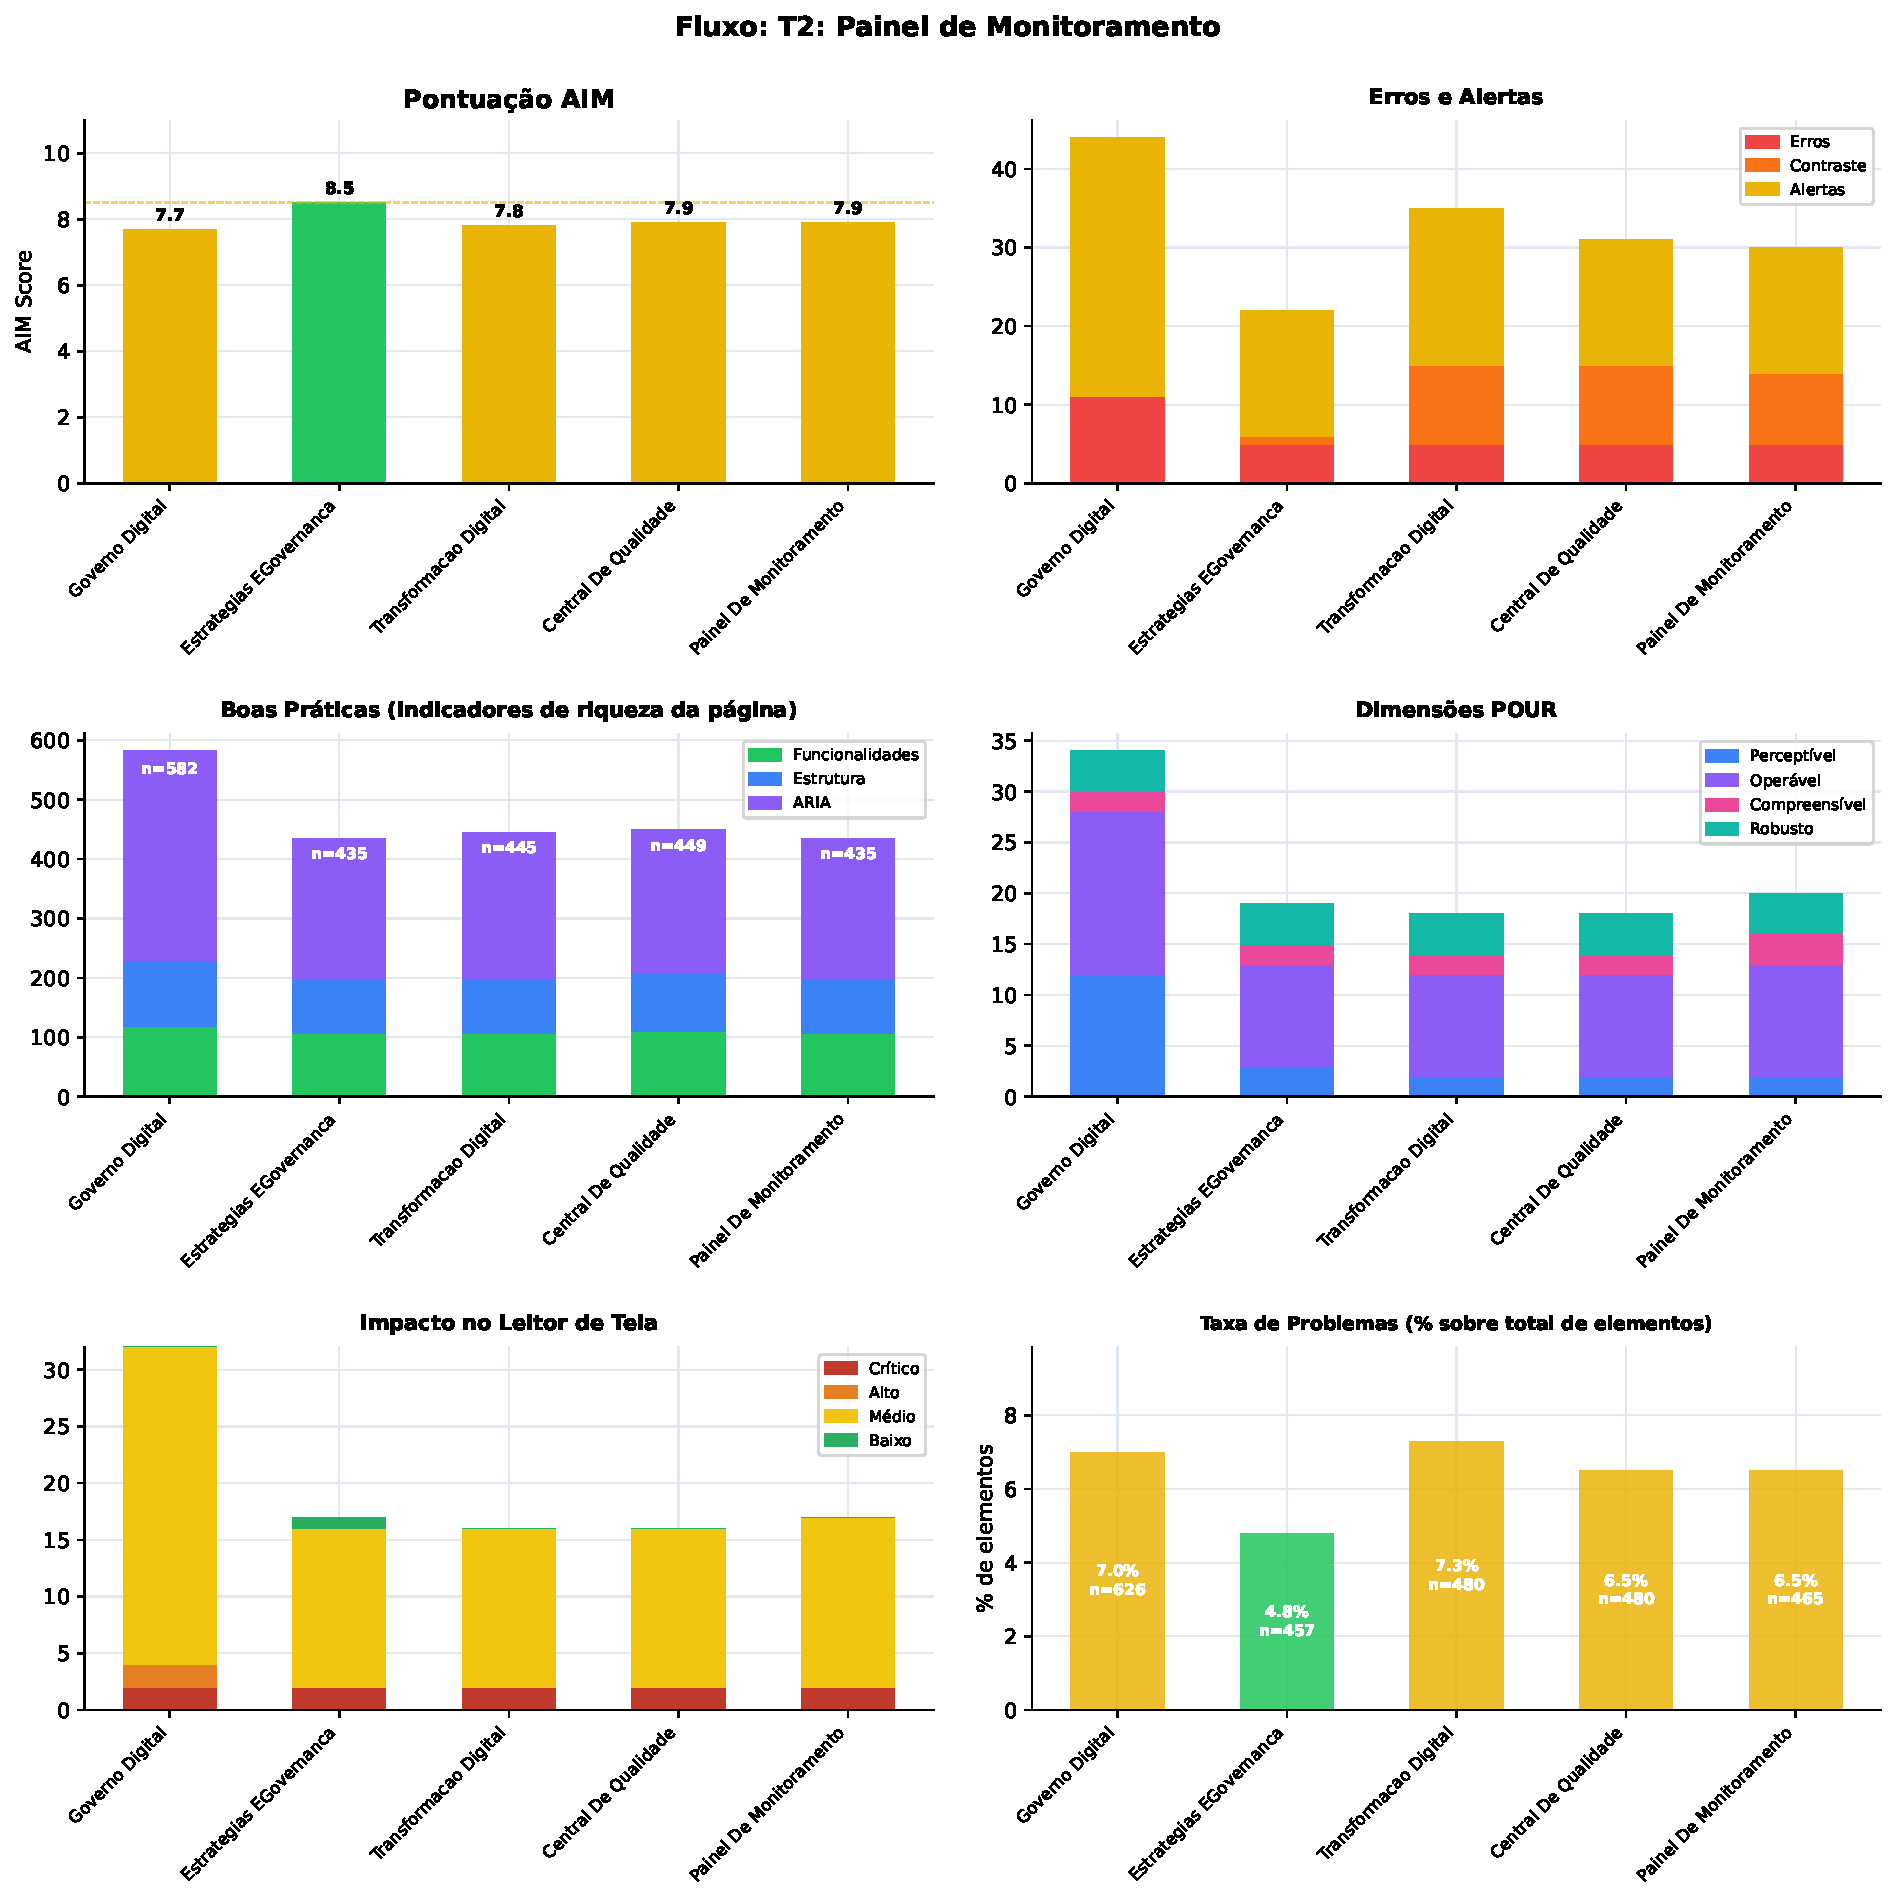
\includegraphics[width=\linewidth]{figures/flow_t2_painel_de_monitoramento}
  \caption{Métricas de acessibilidade — T2: Painel de Monitoramento}
  \label{fig:flow_t2_painel_de_monitoramento}
\end{figure}


\subsection{T1: Consulta CPF}

\begin{table}[htbp]
  \centering
  \caption{Métricas por página — T1: Consulta CPF}
  \label{tab:flow_t1_consulta_cpf}
  \small
  \begin{tabular}{lcrrrrrrrrrr}
\toprule
Página & AIM & Elem. & \% prob. & Erros & Contraste & Alertas & Func. & Estrutura & ARIA & LS Crít. & LS Méd. \\
\midrule
Inicio Consultar Cadastro CPF & 8.500000 & 425 & 5.600000 & 6 & 0 & 18 & 111 & 51 & 239 & 2 & 10 \\
Formulario Consulta CPF & 5.400000 & 62 & 61.300000 & 5 & 11 & 22 & 6 & 16 & 2 & 2 & 7 \\
comprovante Situacao CPF & 6.000000 & 55 & 65.500000 & 4 & 9 & 23 & 8 & 11 & 0 & 1 & 7 \\
\bottomrule
\end{tabular}
\end{table}


\begin{figure}[htbp]
  \centering
  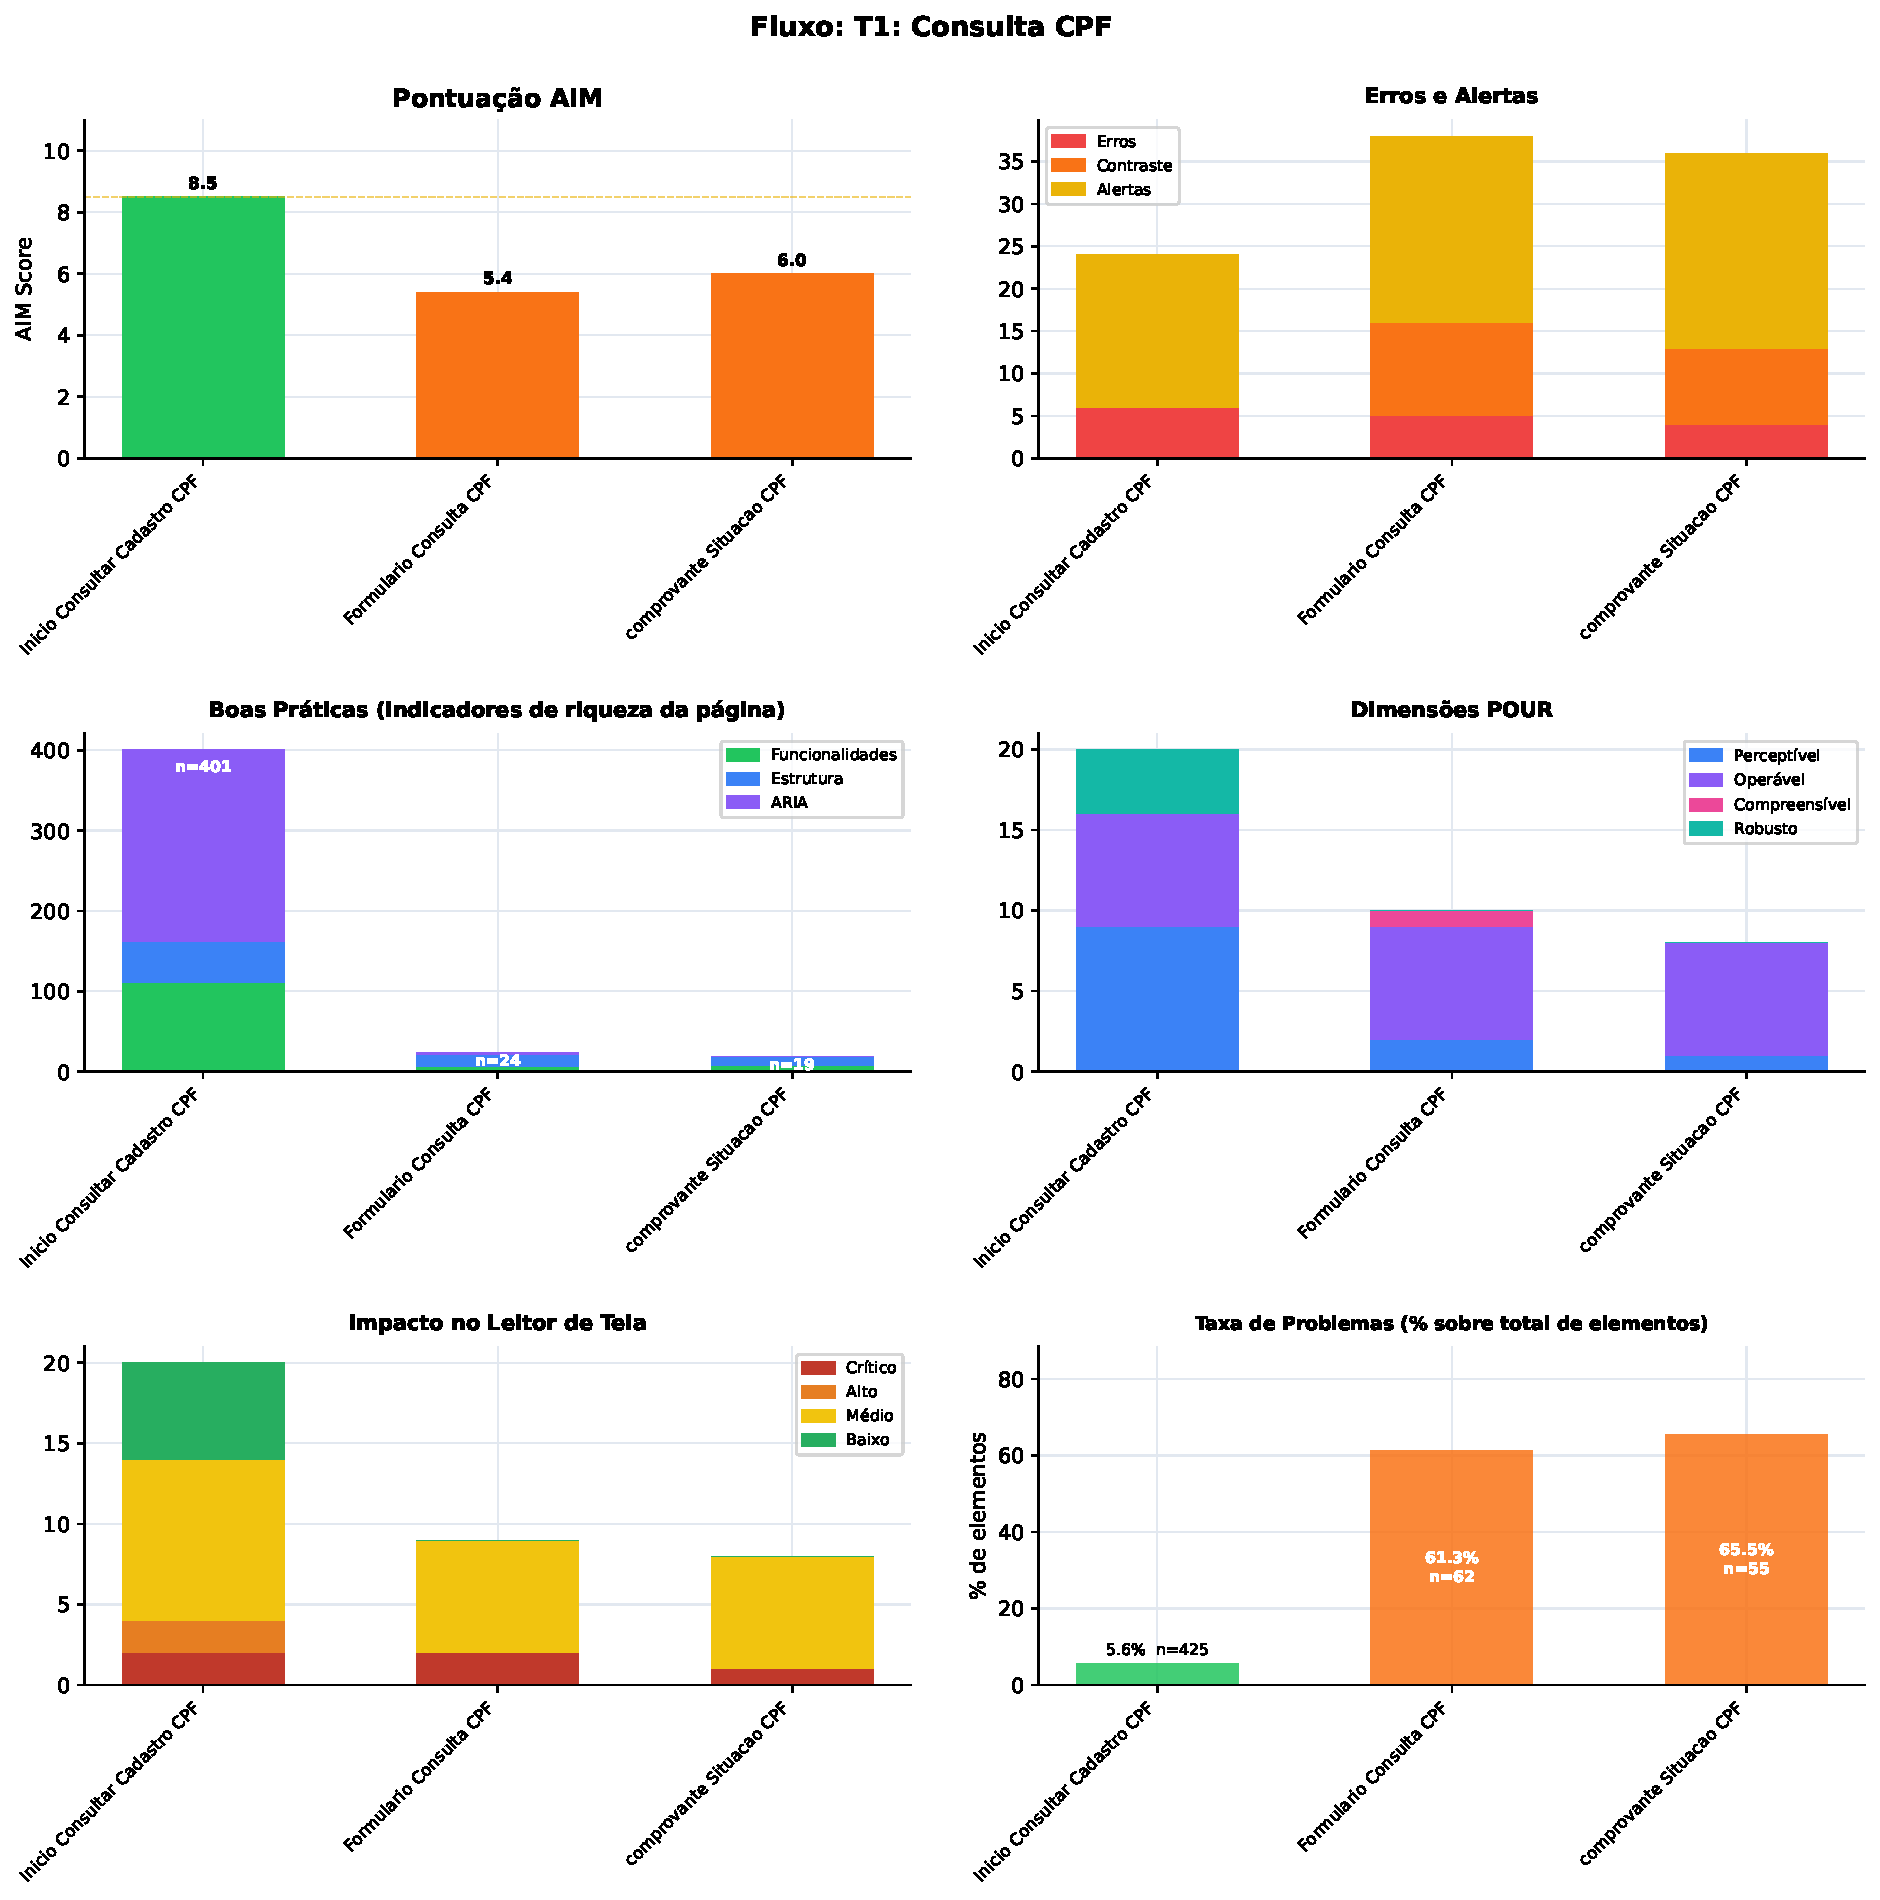
\includegraphics[width=\linewidth]{figures/flow_t1_consulta_cpf}
  \caption{Métricas de acessibilidade — T1: Consulta CPF}
  \label{fig:flow_t1_consulta_cpf}
\end{figure}


%% ─────────────────────────────────────────────────────────────
\section{Principais Problemas de Acessibilidade}

\begin{table}[htbp]
  \centering
  \caption{Principais 15 problemas de acessibilidade — todos os fluxos}
  \label{tab:top_issues}
  \small
  \begin{tabular}{lcrrcclc}
\toprule
 & Problema & Tipo & Total & Pág. & WCAG & Nível & POUR & Imp. LS \\
\midrule
1 & Very low contrast & Contraste & 147 & 10 & --- &  & --- & --- \\
2 & Very small text & Alerta & 89 & 6 & --- &  & --- & --- \\
3 & Accesskey & Alerta & 78 & 16 & 2.1.4 & A & Operable & Médio \\
4 & Redundant link & Alerta & 65 & 13 & 2.4.4 & A & Operable & Médio \\
5 & Empty link & Erro & 58 & 15 & --- &  & --- & --- \\
6 & Redundant title text & Alerta & 53 & 10 & --- &  & --- & --- \\
7 & Noscript element & Alerta & 24 & 13 & 4.1.2 & A & Robust & Médio \\
8 & A nearby image has the same alternative text & Alerta & 22 & 14 & --- &  & --- & --- \\
9 & Empty button & Erro & 22 & 1 & --- &  & --- & --- \\
10 & Broken ARIA reference & Erro & 22 & 11 & 4.1.2 & A & Robust & Crítico \\
11 & Justified text & Alerta & 21 & 4 & 1.4.8 & AAA & Perceivable & Baixo \\
12 & Missing alternative text & Erro & 19 & 5 & 1.1.1 & A & Perceivable & Crítico \\
13 & YouTube video & Alerta & 15 & 5 & 1.2.2 & A & Perceivable & Médio \\
14 & Possible heading & Alerta & 15 & 4 & --- &  & --- & --- \\
15 & Link to PDF document & Alerta & 12 & 6 & 2.4.4 & A & Operable, Understandable & Médio \\
\bottomrule
\end{tabular}
\end{table}


\begin{figure}[htbp]
  \centering
  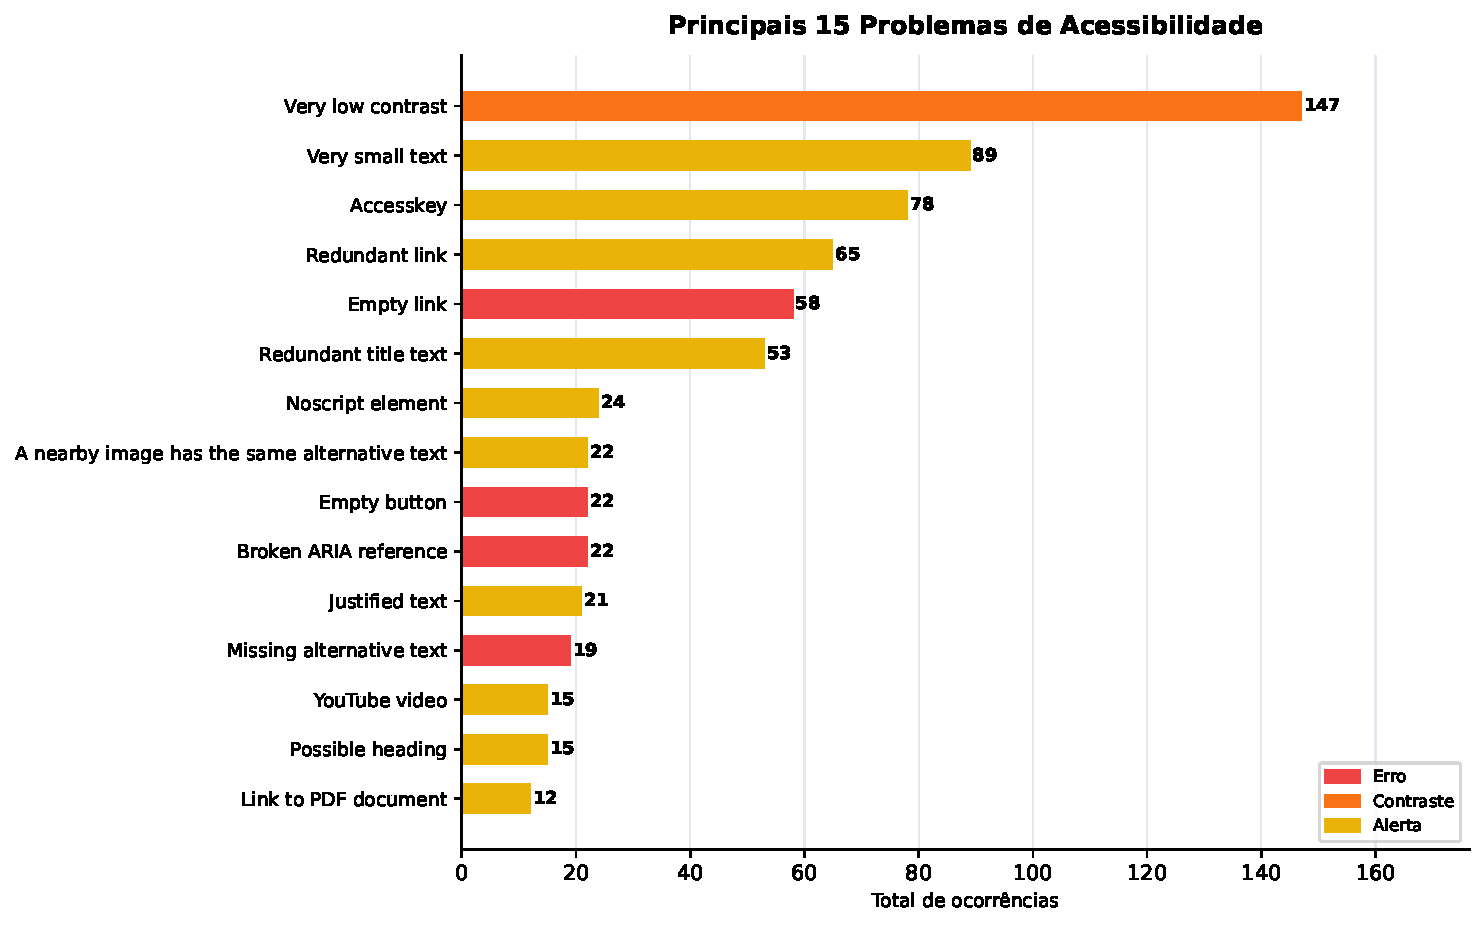
\includegraphics[width=\linewidth]{figures/top_issues}
  \caption{Principais 15 problemas de acessibilidade por número total de
           ocorrências em todos os fluxos.}
  \label{fig:top_issues}
\end{figure}

\end{document}
